\documentclass[12pt]{article}
\usepackage{fullpage}
\usepackage{graphicx}
\usepackage{amsmath}
\usepackage{url}
\usepackage{parskip}
\usepackage[margin=15pt,font=small,labelfont=bf,labelsep=endash]{caption}


%TYPESETTING
\newcommand{\smat}{\left( \begin{matrix}} %start matrix
\newcommand{\emat}{\end{matrix} \right)} %end matrix

\newcommand{\bea}{\begin{eqnarray*}} %begin unnumbered equation array
\newcommand{\eea}{\end{eqnarray*}} %end unnumbered equation array

\newcommand{\beq}{\begin{equation}} %begin numbered equation that I won't be referring back to
\newcommand{\be}[1]{\begin{equation}\label{#1}} %begin numbered equation with a label so I can refer back to it
\newcommand{\ee}{\end{equation}} %end numbered equation

\newcommand{\bskip}{\bigskip\noindent} %new non-indented paragraph, spaced from previous

%FORMULA MACROS
\renewcommand{\(}{\left(}
\renewcommand{\)}{\right)}
\renewcommand{\Im}{\operatorname{Im}}
\renewcommand{\Re}{\operatorname{Re}}

\newcommand{\E}{\mathbf{E}}
\renewcommand{\H}{\mathbf{H}}
\renewcommand{\k}{\mathbf{k}}
\newcommand{\hatk}{\hat{\mathbf{k}}}
\renewcommand{\S}{\mathbf{S}}
\renewcommand{\r}{\mathbf{r}}
\newcommand{\x}{\hat{\mathbf{x}}}
\newcommand{\y}{\hat{\mathbf{y}}}
\newcommand{\z}{\hat{\mathbf{z}}}
\begin{document}

\section{Introduction}

Written by Steve Byrnes, 2012. Please email me any feedback. My website is \url{http://sjbyrnes.com} . Last update/upload: 14 December 2012.

This is a group of programs written in Python / NumPy for simulating light propagation in planar multilayer thin films, including the effects of multiple internal reflections and interference, using the ``Transfer Matrix Method''. It can also simulate combinations of thin and thick films (e.g. a thick piece of glass with a multi-layer antireflection coating on one side and a mirror on the other side), or purely thick films.

In addition to calculating how much light is transmitted and reflected, the program can calculate, at any given point in the structure, how much light is being absorbed there. This is a very important feature for solar-cell modeling, for example.

It can also calculate the parameters measured in ellipsometry.

There are three files: \verb=tmm_core.py= contains all the main programs, \verb=examples.py= contains a few example calculations to get you started, and \verb=tests.py= contains a number of programs that perform various tests and consistency checks to confirm that everything is coded and running correctly. There is also the standard \verb=__init__.py=, the home of the main \verb=tmm= namespace, into which are imported all the \verb=tmm_core= functions.

I did not compile any API documentation (list of functions and parameters), except the source code itself. You should read \verb=tmm_core.py=: I tried hard to put complete information into each function docstring about what the function does and how to use it. Also look at \verb=examples.py= to see examples of various kinds of calculations and plots.

\section{Other people's programs}

There are many other free (and non-free) programs that do some or all of what this program does. Here are the ones I know of:
\begin{itemize}
\item \url{http://empy.sourceforge.net/}
\item \url{http://www-swiss.ai.mit.edu/~jaffer/FreeSnell/}
\item \url{http://optics.unige.ch/alexey/reffit.html}
\item \url{http://www.ub.edu/optmat/programs.html}
\item \url{http://www.luxpop.com/}
\item \url{http://thinfilm.hansteen.net/}
\item \url{http://www.lightmachinery.com/optical-calculations.php}
\item \url{http://pypi.python.org/pypi/openTMM}
\item \url{http://www.stanford.edu/group/mcgehee/transfermatrix/}
\end{itemize}

I have done a few consistency checks between my program and others. They tend to agree perfectly except in the tricky (and somewhat unusual) case of calculating reflected power or transmitted power when the semi-infinite incoming and/or outgoing medium has a complex index of refraction. [However, I'm confident that my formulas are correct, see below.]

\section{Installation}

Requires SciPy and NumPy to run. The ``examples'' also use Matplotlib. Written in Python 2.7. It is very likely compatible with Python 2.6 and perhaps earlier, but I haven't checked. Install via \verb=pip= or just download it directly (it's pure python).

\subsection{Installation for dummies}

If you've never used Python before, getting started can be a bit tricky. See \url{http://sjbyrnes.com/?page_id=67} for installation advice.

You can install this package by typing \verb=pip install tmm= into a terminal / command line. Or, since the package is pure python and requires no setup or compilation, you can just download it directly. Put the \verb=tmm= folder somewhere that Python can find it. (If you're not sure, type \verb=import sys; sys.path= into IPython.)

To get going, try typing the following in IPython (pylab mode):

\begin{verbatim}
>> import tmm.examples
>> tmm.examples.sample1()
\end{verbatim}

A plot should pop up.

\section{Units}

The program implicitly requires a unit of length. You can use any unit, but keep it consistent. For example, if wavelength is given in nanometers, the thicknesses of the layers should also be given in nanometers, and the absorption at a given point will be in (fraction of incoming light power per nanometer of depth).

\section{Theoretical background}

The rest of this document lists the equations that form the basis of the program and explains where they come from. Where possible the equations are based on Bo Sernelius's lecture notes: \url{http://people.ifm.liu.se/boser/elma/} (especially lecture 13).

\section{Wave propagation}

The planar film is assumed to be uniform in the $x$ and $y$ directions, so that surfaces are normal to $\z$. We assume the wavevector is in the x-z plane. (Or just the $z$ direction if it's normal-incidence). The ``forward'' direction (direction that normally-incident incoming light is traveling) is $+\z$.

The electric field at any given point is a superposition of the forward-moving and backwards-moving electromagnetic waves:
$$\E(\r) = \E_f^0 e^{i\k_f\cdot\r} + \E_b^0 e^{i\k_b\cdot\r}$$
(Implicitly, you always multiply by $e^{-i\omega t}$ and  then take the real part.) Here, $\k_f$ and $\k_b$ is the [angular] wavevectors for foward- and backwards-moving waves; $\E_f^0$ and $\E_b^0$ are some constant vectors; and $\E(\r)$ is the complex electric field at any given point $\r$ within a certain layer. The $y$-components of the $\k_f$ and $\k_b$ are zero, by definition of the $x$-axis. The $x$-components of $\k_f$ and $\k_b$ are always  real, because we assume the light intensity is uniform along the $x$ and $y$ directions. However, the $z$ component might be complex, representing a wave that is attenuating as it travels through the stack, due to absorption.

The wavevectors is related to the [complex] index of refraction $n$ by:
$$\k_f = \frac{2\pi n}{\lambda_{vac}}(\z \cos \theta + \x \sin \theta)$$
$$\k_b = \frac{2\pi n}{\lambda_{vac}}(-\z \cos \theta + \x \sin \theta)$$
where $\theta$ is the angle from the normal, $\lambda_{vac}$ is the vacuum wavelength. That means $n \sin \theta$ is always a real number, but $n \cos \theta$ might not be. This is consistent with Snell's law:
$$n_i \sin \theta_i = n_j \sin \theta_j$$
i.e., $n\sin \theta$ should be the same real number in every layer. Snell's law is the same as saying that the component of $\k$ in the $x-y$ plane is the same in any layer.

\section{What is complex refractive index?}

When the refractive index is complex, the imaginary part is sometimes called ``extinction coefficient''. The larger it is, the more light the material absorbs. Negative extinction coefficient corresponds to stimulated emission. Extinction coefficient, like refractive index, is a unitless number It should \emph{NOT} be confused with ``molar extinction coefficient'' or ``mass extinction coefficient'' in chemistry, which are not unitless. [However, if you know one you can figure out the other. See \url{http://en.wikipedia.org/wiki/Mathematical_descriptions_of_opacity} .] For real-world materials, the extinction coefficient, like the refractive index, is different at different frequencies.

Again, with the conventions used here, $\Im n>0$ means absorption and $\Im n<0$ means stimulated emission.

\section{Explicit $\E$, $\H$, and $\k$ for s-polarization and p-polarization}

As usual, $s$-polarization is where the $\E$-field points in the $y$-direction, and $p$-polarization is where the $\H$-field points in the $y$-direction. (There is no difference between $s$ and $p$-polarization for normal-incident light.

Maxwell's equations imply that $\H = \frac{\mu}{\omega}\k \times \E$ for a plane wave. [This works even if $\k$ and/or $\E$ is a complex vector.] Therefore the explicit $\E,\H,\k$ are:

\begin{center} {\bf \underline{s-polarization}}\footnote{I'm using Sernelius's convention, where a forward- and backward-moving s-polarized wave have the same amplitude sign if their $E$-fields point in the same direction. I am also assuming throughout that $\mu$, the magnetic permeability, is approximately equal in each layer.}
 \end{center}
$$\E_f = E_f \y, \quad \E_b = E_b \y$$
$$\k_f =\frac{2\pi n}{\lambda_{vac}}\( \cos \theta \z + \sin \theta \x\), \quad \k_b = \frac{2\pi n}{\lambda_{vac}}\(- \cos \theta \z + \sin \theta \x\)$$
$$\H_f \propto  n E_f \( - \cos \theta \x +  \sin \theta \z\), \quad \H_b \propto n E_b\( \cos \theta \x + \sin \theta \z\)$$

Now with p-polarization,
\begin{center} {\bf \underline{p-polarization}}\footnote{I'm using Sernelius's convention, where a forward- and backward-moving p-polarized wave have the same amplitude sign if their $H$-fields point in the same direction. I am also assuming throughout that $\mu$, the magnetic permeability, is approximately equal in each layer.} \end{center}
$$\k_f =\frac{2\pi n}{\lambda_{vac}}\( \cos \theta \z + \sin \theta \x\), \quad \k_b = \frac{2\pi n}{\lambda_{vac}}\(- \cos \theta \z + \sin \theta \x\)$$
$$\E_f = E_f(-\sin \theta \z +  \cos \theta \x), \quad \E_b = E_b(- \sin \theta \z -  \cos \theta \x)$$
$$\H_f \propto n E_f \y, \quad \H_b \propto n E_b \y$$

\section{Single-interface reflection and transmission amplitudes, sign convention}

If you have the interface between two layers 1 and 2, and shine light from 1, then you have the incident amplitude ($E_f$ on the layer 1 side), the reflected amplitude ($E_b$ on the layer 1 side), and the transmitted amplitude ($E_f$ on the layer 2 side). The reflection coefficient $r$ is the ratio of reflected amplitude to incident amplitude, and the transmission coefficient $t$ is the ratio of transmitted amplitude to incident amplitude.

The sign of $r$ depends on what it means for $E_b$ and $E_f$ to have the same sign versus opposite sign. I'm using Sernelius's convention (see previous section and footnotes). In other references, other conventions are used, and therefore $r$ might have the opposite sign. Beware!

The equations for $r$ and $t$ (``The Fresnel Equations'') are as given in Sernelius: Traveling from medium 1 into medium 2:
$$r_s = \frac{n_1 \cos \theta_1 - n_2 \cos \theta_2}{n_1 \cos \theta_1 + n_2 \cos \theta_2} \quad , \quad r_p = \frac{n_2 \cos \theta_1 - n_1 \cos \theta_2}{n_2 \cos \theta_1 + n_1 \cos \theta_2}$$
$$ t_s = \frac{2n_1 \cos \theta_1}{n_1 \cos \theta_1 + n_2 \cos \theta_2} \quad , \quad t_p = \frac{2n_1 \cos \theta_1}{n_2 \cos \theta_1 + n_1 \cos \theta_2}$$


\section{Amplitudes for multilayer thin films}

\begin{figure}[htb]
\centering
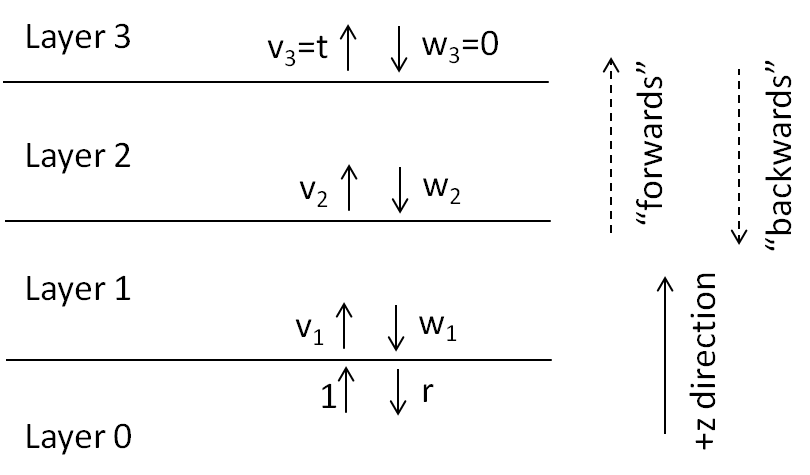
\includegraphics[width=0.5\textwidth]{vwdefn.png}
\caption{Sample stack with $N=4$ (two finite layers between two semi-infinite layers). The labels next to the small arrows indicate wave amplitudes.\label{vwdefn}}
\end{figure}

Now we have $N$ materials, numbered $0,1,\ldots,N-1$, where the first (``0'') and last (``$N-1$'') layer are semi-infinite. Light with amplitude 1 is entering towards layer 1 (Fig.~\ref{vwdefn}).

At the interface between the $(n-1)$st and $n$th material, let $v_n$ be the amplitude of the wave on the $n$th side heading forwards (away from the boundary), and let $w_n$ be the amplitude on the nth side heading backwards (towards the boundary). (Fig.~\ref{vwdefn}.) (($v_0,w_0$) are undefined, while $v_{N-1}=t$ and $w_{N-1}=0$.) Then
$$\smat v_n \\ w_n \emat = M_n \smat v_{n+1}\\w_{n+1}\emat$$
where\footnote{My $M$'s are a bit different than Sernelius's, because I'm using $v$ and $w$, the wave amplitudes just \emph{after} an interface, while Sernelius is using $x$ and $y$, the wave amplitudes just \emph{before} an interface.}
$$M_n = \smat e^{- i \delta_n} & 0 \\ 0 & e^{i \delta_n} \emat \smat 1 & r_{n,n+1} \\ r_{n,n+1} & 1 \emat \frac{1}{t_{n,n+1}}$$
for $n=1,\ldots,N-2$. Now we want the matrix relating the waves entering the structure to the waves exiting, i.e.:
$$\smat 1 \\ r \emat = \tilde{M} \smat t \\ 0 \emat.$$
$\tilde{M}$ is given by:
$$\tilde{M} = \frac{1}{t_{0,1}} \smat 1 & r_{0,1} \\ r_{0,1} & 1 \emat M_1 M_2 \cdots M_{N-1}$$
Combining these two equations allows $r$ and $t$ to be written in terms of the four entries of the matrix $\tilde{M}$:
$$\smat 1\\r \emat = \smat \tilde{M}_{00} & \tilde{M}_{01} \\ \tilde{M}_{10} & \tilde{M}_{11} \emat \smat t \\ 0 \emat$$
$$t = 1/\tilde{M}_{00}, \quad r = \tilde{M}_{10}/\tilde{M}_{00}$$
Incidentally, at this point, it is straightforward to calculate $v_n$ and $w_n$ for every $n$.

\section{Calculating Poynting vector}

\begin{figure}[htb]
\centering
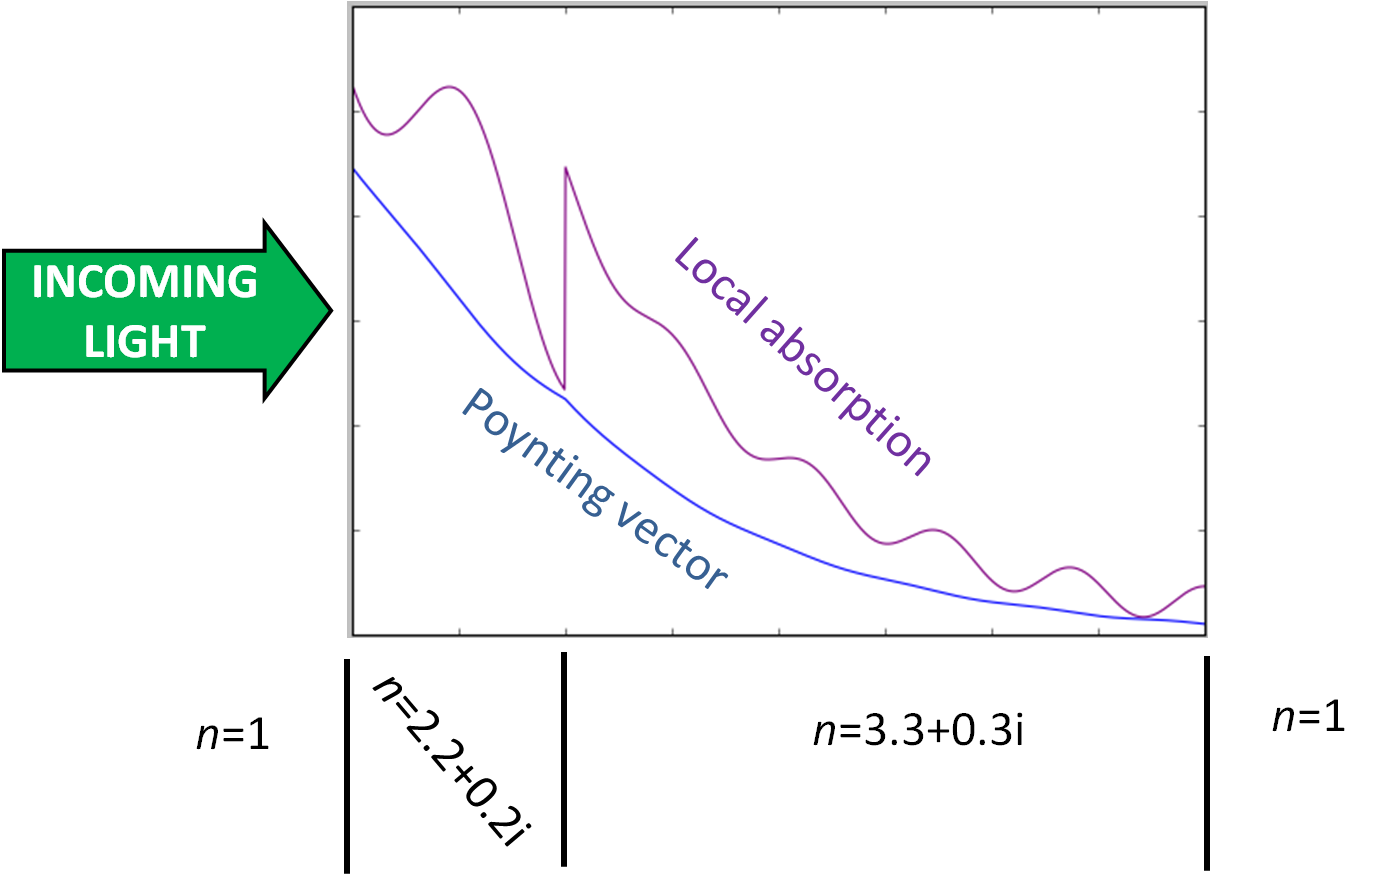
\includegraphics[width=0.5\textwidth]{spatiallyresolvedexample.png}
\caption{Sample calculation of local absorption and Poynting vector in a two-layer structure with air on both sides (refractive indices written below the graph).\label{spatiallyresolvedexample}}
\end{figure}

The next few sections relate to power flows and power absorption: The goal is to be able to generate graphs like Fig.~\ref{spatiallyresolvedexample}. The relevant equations are somewhat hard to find (without typos) in the literature, but I verified them by various consistency checks, such as continuity across interfaces when appropriate, agreement with $R$ and $T$ in simple cases, etc.

I will start by deriving the expression for the normal component of the Poynting vector $\S$, i.e. $\S\cdot\z$. This dot-product is called ``poyn'' in the program. It represents the net power flowing forward through the structure at a given point. It is unitless, because it is expressed as a fraction of the total incoming power. Start with s-polarization, using the expressions from a previous section:

\bea
\E &=& E_f \y + E_b \y \\
\H &\propto& n E_f \( - \cos \theta \x +  \sin \theta \z\) + n E_b\( \cos \theta \x + \sin \theta \z\) \\
\S \cdot \z &=& \frac12 \Re[ \z \cdot (\E^* \times \H)] \propto \Re[(E_f^*+E_b^*) (E_f - E_b)n \cos \theta]\eea
After normalizing to incident power:
$$\text{s-polarization:} \qquad \S \cdot \z = \frac{\Re\left[ (n) (\cos \theta) (E_f^* + E_b^*) (E_f - E_b)\right]}{\Re\left[ n_0 \cos \theta_0\right] }$$

Next, p-polarization:
\bea
\E &=& E_f(-\sin \theta \z +  \cos \theta \x) + E_b(- \sin \theta \z -  \cos \theta \x) \\
\H &\propto& n E_f \y + n E_b \y \\
\S \cdot \z &=& \frac12\Re[ \z \cdot (\E^* \times \H)] \propto \Re[(\cos \theta)^*(E_f^*-E_b^*) (E_f + E_b)n ]\eea
After normalizing to incident power:
$$\text{p-polarization:} \qquad \S \cdot \z = \frac{\Re\left[ (n) (\cos \theta^*) (E_f + E_b) (E_f^* - E_b^*)\right]}{\Re \left[ n_0 \cos \theta_0^* \right]}$$

\section{$T$ (transmitted intensity)}

To get the formula for $T$, the fraction of power transmitted, we just apply the Poynting vector formula above to the special case of the final medium, where $E_b=0$ (no light is flowing back towards the material from the other side):
$$\text{s-polarization:} \qquad T = |t|^2\frac{ \Re\left[ n \cos \theta\right]}{\Re \left[ n_0 \cos \theta_0 \right] }$$
$$\text{p-polarization:} \qquad T = |t|^2\frac{ \Re\left[ n \cos \theta^* \right]}{\Re \left[ n_0 \cos \theta_0^* \right] }$$
where $T$ is the fraction of power transmitted and $t=E_f/E_0$ is the transmission amplitude.\footnote{In some references, the complex conjugation for p-polarization is omitted, but I'm very confident it's correct. Usually the incident and final media are non-absorbing, e.g. air, so $\cos \theta$ is real and it doesn't matter whether you conjugate $\theta$ or not.}

\section{$R$ (reflected intensity) and ``power entering''}

The formula for $R$ is just what you expect:
$$R=|r|^2$$

An interesting thing---which had me confused at first---is that the power entering the first layer of the stack (called \verb=power_entering= in the program) is \emph{not} necessarily equal to $1-R$, as one would expect (energy 1 moving forwards, minus energy $R$ moving backwards). Likewise, it is possible to have $R+T\neq 1$ for an interface between two semi-infinite media. This strange situation only comes up when the starting semi-infinite medium is absorbing. Why does this happen? To find out, read Appendix~\ref{appendixR}!

Quick summary of Appendix A: For an interface between two semi-infinite media, \verb=power_entering= is always equal to $T$. When the incident semi-infinite medium has real refractive index, \verb=power_entering= is always equal to $1-R$. The difference between \verb=power_entering= and $1-R$ is related to an excess or deficit of absorption just before the interface, arising from interference between the incoming and reflected waves. $R$ is defined not by the power that \emph{doesn't} enter the medium, but by the power that \emph{does} enter the reflected wave. See Appendix~\ref{appendixR}.

\section{Absorbed energy density}
Next, absorbed energy density at a given depth. In principle this has units of [power]/[volume], but we can express it as a multiple of incoming light power density on the material, which has units[power]/[area], so that absorbed energy density has units of 1/[length]. This is the negative derivative (with respect to distance) of the ``Poynting'' expressions above. Differentiating is straightforward, using $E_f(z) \propto e^{i k_z z}$ and $E_b(z) \propto e^{-i k_z z}$. (Here, $k_z=2\pi n\cos\theta/\lambda_{vac}$.) The result is:
\bea
\text{s-polarization:} \qquad a(z) &=& \frac{|E_f+E_b|^2 \Im\left[ n \cos(\theta) k_z\right] }{\Re\left[ n_0 \cos \theta_0 \right] } \\
\text{p-polarization:} \qquad a(z) &=& \frac{\Im\left[ n \cos(\theta^*)\(k_z|E_f-E_b|^2-k_z^*|E_f+E_b|^2\)\right]}{\Re \left[ n_0 \cos \theta_0^* \right] }
\eea

Within a given layer, absorption is an analytical function:
$$a(z) = A_1e^{2 z \Im(k_z)} + A_2e^{-2 z \Im(k_z)} + A_3e^{2iz\Re(k_z)} + A_3^* e^{-2iz \Re(k_z)}$$
where:
\bea
\text{s-polarization}: A_1 &=& \frac{\Im\left[ n \cos(\theta) k_z\right] }{\Re\left[ n_0 \cos \theta_0 \right] }|w|^2\\
A_2 &=& \frac{\Im\left[ n \cos(\theta) k_z\right] }{\Re \left[ n_0 \cos \theta_0 \right] }|v|^2\\
A_3 &=& \frac{\Im\left[ n \cos(\theta) k_z\right] }{\Re \left[ n_0 \cos \theta_0 \right] }vw^*\\
\text{p-polarization}: A_1 &=& \frac{2\Im\left[ k_z\right] \Re\left[ n \cos(\theta^*)\right] }{\Re \left[ n_0 \cos \theta_0^* \right] } |w|^2\\
A_2 &=& \frac{2\Im\left[ k_z \right] \Re \left[ n \cos(\theta^*)\right] }{\Re \left[ n_0 \cos \theta_0^* \right] } |v|^2\\
A_3 &=& \frac{2\Re\left[ k_z \right] \Im \left[ n \cos(\theta^*)\right] }{\Re \left[ n_0 \cos \theta_0^* \right] } vw^*
\eea
where $v = E_f(0)$ and $w=E_b(0)$.

\section{Branch cuts \label{branchcuts}}

Snell's law gives $\theta_i = \arcsin(n_0 \sin(\theta_0)/n_i)$. However, the arcsin function is ambiguous--it has branch cuts in the complex plane. How do we get the right $\theta$??

There are actually only two non-equivalent choices. If $\theta$ is one solution, then $\pi-\theta$ is the other. You may recognize that we are choosing which of the two waves in medium $i$ is called ``forward-traveling'' and which one is called ``backward-traveling''. How do we make the right choice??

Good news: In the intermediate, finite-thickness layers, the choice actually doesn't matter. We solve for \emph{both} the forward- and backward-traveling waves, so it doesn't matter which wave has which name. The two choices of $\theta_i$ will switch $v_i$ with $w_i$, but won't affect observable quantities like reflectance, absorption, etc.

Bad news: The choice of $\theta$ versus $\pi-\theta$ \emph{does} matter very much in the starting semi-infinite layer (where the ``forward-traveling'' wave amplitude is set to 1), and in the final semi-infinite layer (where the ``backwards-traveling'' wave amplitude is set to 0). In these layers, we need to choose $\theta$ correctly.

I've only checked the case I care about, $\Re n>0$ and $\Im n \geq 0$. In that case, the naive calculation (using the default behavior of arcsine) gives the correct answer for all cases, in both Python\footnote{Note: For python, you need to use the arcsine function in SciPy, not the one in NumPy, so that when you calculate the arcsine of a real number greater than 1, e.g. total internal reflection, you get a complex angle instead of nan. Or, you can use NumPy arcsine if you cast its argument to complex.} and Mathematica. I think I checked this pretty carefully, see the appendix (Section~\ref{appendixbranchcuts}) for details.

In more specialized cases, like negative-index materials ($\Re n <0$) or stimulated-emission media ($(\Im n)/(\Re n)<0$), results are not guaranteed! Please check this before using, if your starting or ending layer is one of these!

\section{Thick ``incoherent'' films: Introduction}
That finishes the thin-film part of the program. Next, thick films. Here we are interested in hybrid structures containing both thick and thin layers (or even just thick layers). Light loses its coherence when traveling through the thick layers--i.e., the Fabry-Perot fringes are so close together that they cannot be resolved by the experimental measurement, due to factors such as random thickness variations, propagation angle variations, and/or wavelength variations. Instead of seeing the fringes, you just see the average.

In this program, there are two types of layers: Coherent layers (treated as in the sections above), and incoherent layers. Generally, a layer should be treated as coherent if its thickness is comparable to the light wavelength or smaller, and incoherent if it's much larger than the light wavelength.

As soon as light enters an incoherent layer, its phase information is thrown out, and only its intensity is remembered. The program has no partial coherence, it's all or nothing!

For more on this topic see these references: Harbecke\footnote{\url{http://dx.doi.org/10.1007/BF00697414}} and Katsidis\footnote{\url{http://dx.doi.org/10.1364/AO.41.003978}}. These papers, which I have not read in detail, seem to offer more powerful and general methods than the basic approach I'm using.

\section{Thick ``incoherent'' films: Calculation method}

\begin{figure}[htb]
\centering
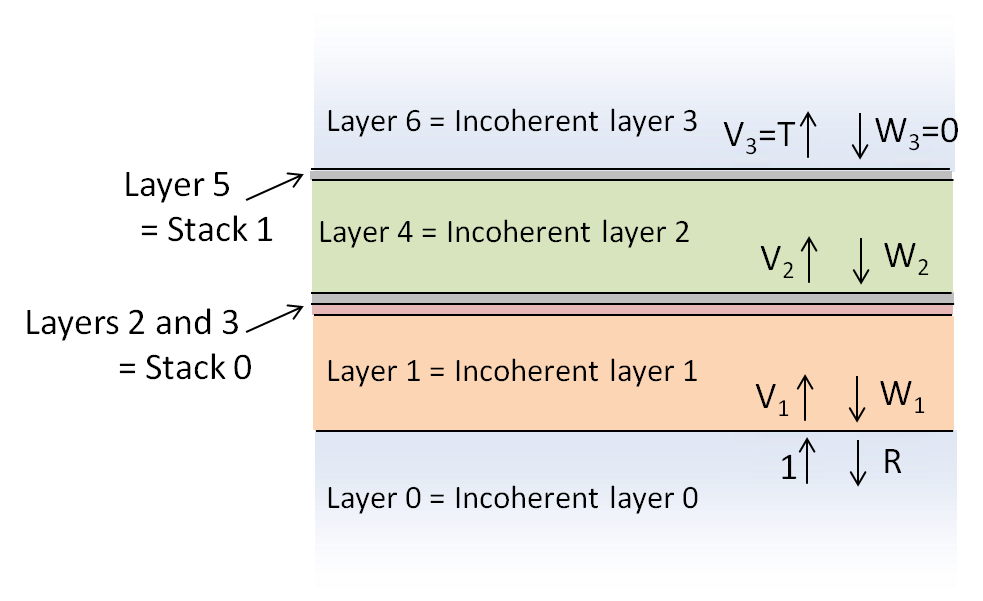
\includegraphics[width=0.5\textwidth]{incoherentfig.png}
\caption{Variable definitions related to the incoherent calculation program. A ``stack'' is one or more consecutive coherent layers. Note the three numbering systems: Each layer has a layer index, each incoherent layer has an incoherent layer index, and each stack has a stack index. $V_i,W_i$ are power flows (note the capital letters, not to be confused with the amplitudes $v_i,w_i$ in Fig.~\ref{vwdefn}).\label{incoherentfig}}
\end{figure}

We have a number of incoherent layers 0,1,...,$N-1$. Let $V_i$ be the forward propagation \emph{intensity} and $W_i$ be the backwards \emph{intensity} at the \emph{beginning} of the $i$th incoherent layer. (Capital letters to distinguish from $v,w$, the amplitudes in the coherent program, see previous section.) Let $X_i$ and $Y_i$ be forward and backwards at the \emph{end} of the $i$th incoherent layer. ($X_i$ and $Y_i$ are not explicitly calculated in the program.) Let $T_{i,j}$ be transmissivity from the $i$th to $j$th incoherent layer (where $j=i\pm 1$, and $R_{i,j}$ the reflectivity. Then:
$$Y_i = X_i R_{i,i+1} + W_{i+1} T_{i+1,i}$$
$$V_{i+1} = X_i T_{i,i+1} + W_{i+1} R_{i+1,i}$$
$$\smat X_i \\ Y_i \emat = \frac{1}{T_{i,i+1}} \smat 1 & -R_{i+1,i} \\  R_{i,i+1} & T_{i+1,i}T_i -  R_{i+1,i}R_{i,i+1} \emat \smat V_{i+1} \\ W_{i+1} \emat.$$
Let $P_i$ be the fraction of light that passes successfully through layer $i$ (in a single pass) without getting absorbed, calculated by
$$P_i = e^{-\alpha d_i}, \quad \alpha = \frac{4\pi \Im[n_i \cos \theta_i]}{\lambda_{vac}}$$
where $d_i$ is the layer thickness. Then:
$$\smat V_i \\ W_i \emat = \smat 1/P_i & 0 \\ 0 & P_i \emat \smat X_i \\ Y_i \emat$$
Define the matrices $L_n$ by
$$L_n =  \frac{1}{T_{i,i+1}} \smat 1/P_i & 0 \\ 0 & P_i \emat \smat 1 & -R_{i+1,i} \\  R_{i,i+1} & T_{i+1,i}T_{i,i+1} -  R_{i+1,i}R_{i,i+1} \emat$$
for $n=1,\ldots,N-1$. Now we want the matrix relating the intensities  entering the structure to the intensities exiting, i.e.:
$$\smat 1 \\ R \emat = \tilde{L} \smat T \\ 0 \emat.$$
Then the formula for $\tilde{L}$ is
$$\tilde{L} = \frac{1}{T_{0,1}} \smat 1 & -R_{1,0} \\  R_{0,1} & T_{1,0}T_{0,1} -  R_{1,0}R_{0,1} \emat L_1 L_2 \cdots L_{N-1} = \smat \tilde{L}_{00} & \tilde{L}_{01} \\ \tilde{L}_{10} & \tilde{L}_{11} \emat$$
$$T = 1/\tilde{L}_{00}, \quad R = \tilde{L}_{10}/\tilde{L}_{00}$$

\section{Thick ``incoherent'' films: Absorption profile, Coherence length}

Absorption as a function of depth is not implemented in the program for incoherent layers (at least for now); this section explains why.

Calculating the absorption profile within an ``incoherent'' layer is not simple to do correctly. If you look up close, the absorption as a function of position would be oscillatory near an interface due to interference between the incoming and outgoing beams; with the oscillations gradually dying down into a smooth exponential farther away from the interface. The ``coherence length'' describes how far from the interface you need to go before the oscillations die down. For example, if the incoherence is caused by using a not-quite-monochromatic light source, the coherence length would be related to the bandwidth of the light.

If you are only interested in calculating the \emph{total} amount of light absorbed in each layer, it turns out that you do not need to know the coherence length!! More precisely, the coherence length does not effect the total absorption in (and transmission through) an incoherent layer under two assumptions (which are usually satisfied): (1) The coherence length is large compared to a wavelength; (2) The coherence length is small compared to the layer thickness.\footnote{The mathematics of this is that when you have sinusoidal oscillations that die away, their integral is independent of the precise decay properties. Mathematically, $\int_0^\infty e^{ikx} e^{-\alpha x} dx = \frac{1}{-ik+\alpha} \approx \frac{1}{-ik}$; the integral is approximately independent of $\alpha$ as long as $\alpha \ll k$, i.e. as long as the decay length is much larger than the oscillation length.}

That's the reason that you are not prompted to input coherence lengths in any of the calculations above.

On the other hand, if you want to calculate absorption as a function of depth in an incoherent layer, you \emph{do} need to know exactly what the coherence length is.

I'm not sure what to do here. Asking users to input the coherence length seems a bad strategy as most people probably wouldn't know what it is. Assuming a coherence length of 0 would give grossly inaccurate results very close to the interfaces, which would be OK in some applications but not others.

Since I cannot think of a good way to do it, absorption as a function of depth is not implemented for incoherent layers. Sorry! If you want to see absorption as a function of depth for an incoherent layer, maybe you can use the coherent program and average over slightly varying thicknesses or wavelengths (as appropriate) to get rid of spurious oscillations.

\newpage

\renewcommand{\thesection}{\Alph{section}}
\setcounter{section}{0}

\section{Appendix: $R$ (reflected intensity) and ``power\_entering''\label{appendixR}}

We obviously expect $R=|r|^2$ here (as usual), and that's correct.

The interesting thing---which had me confused at first---is that the normalized Poynting vector passing through the first interface is \emph{not} necessarily equal to $(1-R)$, as one would expect (energy 1 moving forwards minus energy $R$ moving backwards). Likewise, it is possible to have $R+T\neq 1$ for an interface between two semi-infinite media. This strange situation only comes up when the starting semi-infinite medium is absorbing. Why does this happen?

To get the exact formulas for Poynting vector at the initial interface, called \verb=power_entering= in the program, we just plug into the normal Poynting vector formula with $E_f = 1$ and $E_b = r$, to get:
\begin{center}\underline{s-polarization:}\end{center}
$$\text{power entering} = \frac{\Re \left[ n_0 \cos \theta_0  (1 + r^*) (1 -r) \right] }{\Re \left[ n_0 \cos \theta_0 \right] } = (1-R) + 2 \Im[r]\frac{\Im[n_0 \cos \theta_0]}{\Re[n_0 \cos\theta_0]}$$

\bskip\begin{center}\underline{p-polarization:}\end{center}
$$\text{power entering} = \frac{\Re \left[ n_0 \cos \theta_0^* (1 +r) (1 - r^*) \right] }{\Re \left[ n_0 \cos \theta_0^* \right] } = (1-R) - 2 \Im[r]\frac{\Im[n_0 \cos \theta_0^*]}{\Re[n_0 \cos\theta_0^*]}$$

The first term is what we expect, the second term is strange.

To explain this funny result, start with how $R$ is defined (in the case of an absorbing semi-infinite medium). The most useful and sensible definition---and the one I'm using---is the one shown in Fig.~\ref{Rfig}: You should be able to say the amount of power going into the reflected beam, at a distance $|z|$ from the interface, \emph{after} the beams have spatially separated, by just calculating $R e^{-\alpha |z|}$ where $\alpha$ is the absorption coefficient. (In fact, that exact calculation is a key ingredient in the incoherent calculation.)

\begin{figure}[htb]
\centering
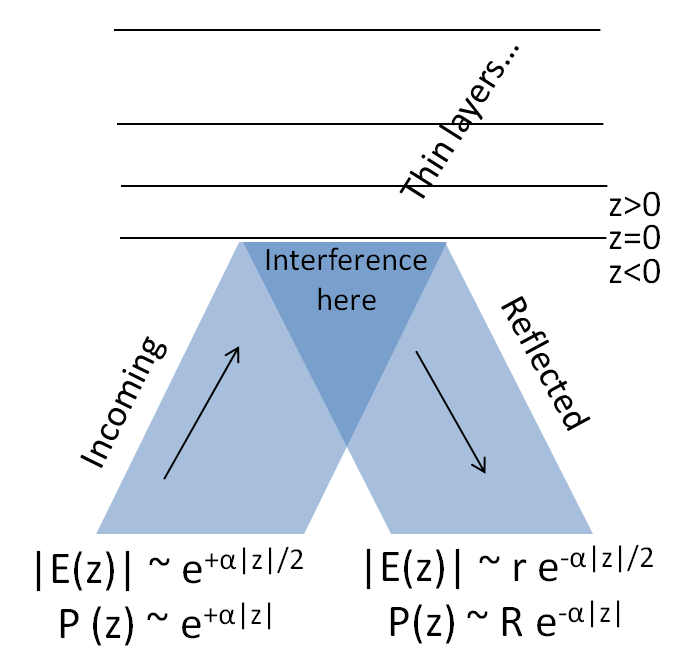
\includegraphics[width=0.5\textwidth]{Rfig.png}
\caption{How the reflected intensity $R$ is defined. Electric field $E$ and power transported $P$ are shown.\label{Rfig}}
\end{figure}

More generally, we naively expect the Poynting vector for $z<0$ in Fig.~\ref{Rfig} to satisfy
\be{Snoninterfered} \S(z)\cdot \z = e^{\alpha |z|} - R e^{-\alpha |z|} \qquad \text{[formula for without wave  interference]} \quad \ee
where the first term comes from the incoming wave and the second term from the reflected wave. It is fine to demand this when the beams do not overlap, but we \emph{CANNOT} use this expression in the ``Interference here'' triangle region of Fig.~\ref{Rfig}. Instead, there is interference between the forward- and backward-moving waves, which causes oscillations in the absorption profile (``hot-spots'' and ``nodes'') (see Fig.~\ref{spatiallyresolvedexample}), so there are corresponding oscillations in the Poynting vector (it's a bit hard to see them in Fig.~\ref{spatiallyresolvedexample} but they're there).  A bit of extra energy is flowing from the nodes to the nearby hot-spots. Thanks to these oscillations, the Poynting vector right at the edge before the start of the structure may not be $1-R$.

If $r$ is real, then there is a node or hot-spot of absorption right at the interface. It turns out that this sort of corresponds to having an integer number of oscillatory cycles, so the oscillations do not effect the power passing through the interface. $R+T=1$ is still valid. But if $r$ is complex, then you have an extra bit of absorption, or deficit of absorption, compared to the non-oscillating baseline expectation of Eq.~(\ref{Snoninterfered}).

Instead of $R+T=1$, the formula is:
$$R+T\pm \text{(extra bit or deficit of absorption from how the oscillations cut off)} = 1$$
Again, this comes from the fact that $R$ is defined by Eq.~(\ref{Snoninterfered}), which is not valid when there is interference.

To verify that $R=|r|^2$ is the correct expression to use, we use the Poynting vector formula, plugged in at an arbitrary depth $z<0$, using $E_f = \exp(2\pi i n z \cos \theta / \lambda_{vac})$ and $E_b = r \exp(-2\pi i n z \cos\theta/\lambda_{vac})$. I'll just do the s-polarized case:
\bea
\S(z)\cdot\z
&=& \frac{\Re[n_0 \cos \theta_0 (E_f^* + E_b^*)(E_f-E_b)]}{\Re[n_0 \cos \theta_0]}\\
&=& \(e^{-4\pi z \Im[n_0 \cos \theta_0]/\lambda_{vac}}-|r|^2 e^{+4\pi z \Im[n_0 \cos \theta_0]/\lambda_{vac})}\) \; +\\
&\;& + \( \; 2\frac{\Im[n_0 \cos\theta_0]}{\Re[n_0 \cos \theta_0]} \Im [r e^{4\pi i z\Re[n_0  \cos \theta_0]/\lambda_{vac}}] \)\\
\eea
The first term corresponds exactly to Eq.~(\ref{Snoninterfered}) with $R=|r|^2$, and the second term is a sinusiodal oscillation corresponding to interference. When the beams stop overlapping (i.e., below the triangle in Fig.~\ref{Rfig}), the oscillation term goes away but the other term remains.

In the program, I use the variable ``\verb=power_entering='' to describe the net power entering the structure, i.e. the Poynting vector at the front of the first layer. For an interface between two semi-infinite media with light coming from just one side, \verb=power_entering= is always equal to $T$. When the incident semi-infinite medium has real refractive index, \verb=power_entering= is always equal to $1-R$.

\subsection{Accounting for this effect in the incoherent calculation}

One of the things I want to compute in the incoherent calculation is how much light gets absorbed in each layer. Part of that absorption is the ``extra'' absorption due to the oscillation cut-off at the interface.

At the interface between two incoherent layers, say 0 and 1, let's say the power flows on the two sides are $P_{f,0},P_{f,1},P_{b,0},P_{b,1}$, where f and b stand forward-moving and backward-moving. The important thing to remember is that the net power actually crossing the interface is \emph{exactly} $P_{f,0}T_{01} - P_{b,1}T_{10}$. Why? Because the transmitted light beams have no funny corrections due to oscillations; they have  nothing to \emph{coherently} interfere with them.

Therefore, the ``extra'' absorption near the interface, not accounted for in the exponential decay of the waves, is exactly equal to
$$(P_{f0}-P_{b0}) - (P_{f0}T_{01} - P_{b1}T_{10}) = P_{f0}(1-R_{01}-T_{01})$$
extra near-interface absorption on the 0 side, and likewise
$$P_{b1}(1-R_{10}-T_{10})$$
extra near-interface absorption on the 1 side.

\section{Appendix: Branch cuts \label{appendixbranchcuts}}

Snell's law gives $\theta_i = \arcsin(n_0 \sin(\theta_0)/n_i)$. However, the arcsin function is ambiguous--it has branch cuts. How to get the right $\theta$?? Remember here, $n_i$ may be an arbitrary complex number, ideally the program will work even for unusual cases like negative-index materials ($\Re n <0$) or stimulated-emission media ($\Im n<0$).

Actually, we never care about $\theta$ itself, just $\sin \theta$ and $\cos \theta$. The sine has no ambiguity:
$$\sin \theta_i = \frac{n_0\sin \theta_0}{n_i}$$
The cosine is more problematic, because there are two choices consistent with Snell's law:
$$\cos \theta_i = \pm \frac{1}{n_i} \sqrt{n_i^2 - (n_0 \sin \theta_0)^2}$$
Do we want the $+$ or $-$?? In other words, we can pick between two angles $\theta$ and $\pi-\theta$.

See Section~\ref{branchcuts} for an explanation of what the choice \emph{really} means, and more importantly, why it only matters in the starting and ending semi-infinite layers, but doesn't matter in the intermediate, finite-thickness layers.

\subsection{Case that $\Im n>0, \quad \Re n > 0$}

For an absorbing material ($\Im n > 0$), a clear requirement is that $\Im(n \cos \theta)>0$. That way, $ \Im k_z > 0$, so the $E_f$ wave in the medium decays rather than amplifying. Another clear requirement is that $R>1$ or $T<0$ cannot occur. This translates to $\Re[n \cos\theta]\geq 0$ for s-polarization and $\Re[n \cos \theta^*]\geq 0$ for p-polarization. This amounts to the same thing as saying that the Poynting vector associated with an $E_f$ wave should point forward not backwards.

Important question: Are these two ``clear requirements'' consistent with each other. Yes!

{\bf Theorem:} If we choose the $\theta$ with $\Im(n \cos \theta)>0$, then it will also be true that $\Re[n \cos\theta] > 0$.

{\bf Proof:} As above,
$$n_i \cos \theta_i = \pm \sqrt{n_i^2 - (n_0 \sin \theta_0)^2}$$
Given that $\Im n_i>0$ and $\Re n_i > 0$, it follows that $\Im n_i^2 >0$. Since $n_0 \sin \theta_0$ is real (the wave intensity is assumed to be uniform in the lateral direction), $(n_i^2 - (n_0 \sin \theta_0)^2)$ also has a positive imaginary part. Therefore, its square root is in the first or third quadrant of the complex plane. That finishes the proof.

{\bf Theorem:} If we choose the $\theta$ with $\Im(n \cos \theta)>0$, then it will also be true that $\Re[n \cos\theta^*] > 0$.

{\bf Proof:}
$$\Re[n_i \cos \theta_i^*] = \Re[n_i^* \cos \theta_i ] = \pm \frac{n_i^*}{n_i}\sqrt{n_i^2 - (n_0 \sin \theta_0)^2}$$
Let $\phi$ with $0<\phi<\pi/2$ be the complex phase of $n_i$. We have
$$\arg \frac{n_i^*}{n_i} = -2\phi$$
Using the fact that $(n_0 \sin \theta_0)^2$ is a nonnegative real number,
$$\arg n_i^2 = 2\phi, \quad 2\phi \leq \arg (n_i^2 - (n_0 \sin \theta_0)^2) < \pi$$
If we choose the square-root with positive imaginary part,
$$\phi \leq \arg \sqrt{n_i^2 - (n_0 \sin \theta_0)^2} < \pi/2$$
Therefore,
$$-\pi/2 < -\phi \leq \arg \left[ \frac{n_i^*}{n_i} \sqrt{n_i^2 - (n_0 \sin \theta_0)^2}\right] < -2\phi+\pi/2 < \pi/2$$
That finishes the proof.

\subsection{Implementation for $\Im n>0, \quad \Re n >0$}
If we use the naive
$$\theta_i = \arcsin(n_0 \sin \theta_0 / n_i)$$
do we get the $\theta_i$ which satisfies
$$\Im(n_i \cos \theta_i)>0$$
in all cases? The answer is ``Yes'', using the default arcsine branch-cut behavior of Python and Mathematica (which are the same). At least, I randomly generated a few million examples and it always worked in both Python and Mathematica, even when $n_0\sin\theta_0<0$.

\subsection{Case that $\Im n=0, \quad \Re n > 0$}
As before,
$$\cos \theta_i = \pm \frac{1}{n_i} \sqrt{n_i^2 - (n_0 \sin \theta_0)^2}$$
There are three cases: Total internal reflection where $n_0\sin\theta_0>n_i$ and $\cos \theta_i$ is pure imaginary; the ordinary case where $n_0 \sin \theta_0 < n_i$ and $\cos \theta_i$ is pure real, and the boundary case where $n_0 \sin \theta_0 = n_i$ and $\cos \theta_i = 0$. The third one has no ambiguity because $\cos \theta_i = -\cos \theta_i$. Let's look at the other two cases.

\subsubsection{Case $\Im n=0, \quad \Re n > 0$, Total internal reflection}
Here, $\Re[n_i \cos\theta_i] = 0$ and $\Re [n_i^* \cos \theta_i^*]=0$, so no need to worry about the sign of the Poynting vector or $R>1$ or $T<0$. The only requirement is that the wave decay rather than amplify, i.e.
$$\Im(n_i \cos \theta_i)>0$$

\subsubsection{Case $\Im n=0, \quad \Re n > 0$, Total internal reflection implementation}
If we use the naive
$$\theta_i = \arcsin(n_0 \sin \theta_0 / n_i)$$
do we get the $\theta_i$ which satisfies
$$\Im(n_i \cos \theta_i)>0$$
in all cases? The answer is ``Yes'', using the default arcsine branch-cut behavior of Python and Mathematica (which are the same). At least, I randomly generated a few million examples and it always worked in both Python and Mathematica, even when $n_0\sin\theta_0<0$.

\subsubsection{Case $\Im n=0, \quad \Re n > 0$, Normal refraction}

Here, $\Im(n_i \cos \theta_i)=0$, so we get no information from whether the wave is decaying or amplifying. The only criterion is $\Re[n_i \cos\theta_i] > 0$ and $\Re [n_i^* \cos \theta_i^*]>0$ (meaning the Poynting vector points forward, $R<1$, $T>0$). In this case it simplifies to $n_i \cos\theta_i > 0$.

\subsubsection{Case $\Im n=0, \quad \Re n > 0$, Normal refraction implementation}
If we use the naive
$$\theta_i = \arcsin(n_0 \sin \theta_0 / n_i)$$
do we get the $\theta_i$ which satisfies
$$n_i \cos \theta_i>0$$
in all cases? The answer is ``Yes'': In both Python and Mathematica, arcsin for real arguments between $-1$ and $1$ returns an angle between $-\pi/2$ and $\pi/2$, i.e. an angle with positive cosine.

\subsection{Stuff I didn't bother with}

I'm not interested in stimulated emission or negative-index metamaterials so I haven't bother to check these cases. Well, I started out of curiosity, enough to convince myself that things make sense, but didn't finish.

\subsubsection{Case that $\Im n<0, \quad \Re n < 0$}

This is \emph{not} stimulated emission, despite $\Im n<0$. It is absorption.[ Remember, with $\Re n<0$, the direction the wave is ``really moving'' (the direction of the Poynting vector) is opposite the direction of the wavevector. When $\Im n<0$, the wave is amplifying in the direction of the wavevector, so it's ``really'' decaying.]

Therefore the required criteria are the same as for ordinary absorbing media with $\Im n>0$ and $\Re n > 0$: $\Im(n \cos \theta)>0$ (the $E_f$ wave decays rather than amplifies),  $\Re[n \cos\theta]\geq 0$ for s-polarization and $\Re[n \cos \theta^*]\geq 0$ for p-polarization (the $E_f$ wave carries energy forwards and $R<1$ and $T>0$.)

If we flip the sign of $n_i$, we do not effect $\sqrt{n_i^2 - (n_0 \sin \theta_0)^2}$, so we do not affect $\cos \theta_i$ (up to a possible sign-flip) nor do we affect $(n_i \cos \theta_i)$ (up to a possible sign-flip). Therefore the proof is exactly the same as before that the two requirements are consistent with each other.

\subsubsection{Case that $\Im n<0, \quad \Re n < 0$ implementation}

Didn't bother to check.

\subsubsection{Case that $\Im n=0, \quad \Re n < 0$}

Didn't bother to check.

\subsubsection{Case of stimulated emission}

Didn't bother to check.


\end{document}
